\documentclass[sigconf]{acmart}

\usepackage{booktabs} % For formal tables
\usepackage{amsmath,amssymb}
\usepackage{array}
% \usepackage{cite}   % importing cite is throwing errors for some reason
\usepackage{color}
\usepackage[inline]{enumitem}
\usepackage{multicol}
\usepackage{float}
% \usepackage[labelfont=bf,textfont=up]{caption}

\usepackage{textcomp}

% Get todos to render properly
\usepackage[obeyFinal]{easy-todo}

% Add package for well rendered quotations
\usepackage{dirtytalk}
\usepackage{hyperref}
\usepackage{graphicx}

\usepackage{lambda}

%package to handle table inputs from separate files
\usepackage{filecontents, catchfile}

% correct bad hyphenation here
\hyphenation{op-tical net-works semi-conduc-tor}

% macro for angled brackets
\newcommand{\brackets}[1]{$\langle$\ignorespaces#1\unskip$\rangle$}
% Copyright
%\setcopyright{none}
%\setcopyright{acmcopyright}
%\setcopyright{acmlicensed}
\setcopyright{rightsretained}
%\setcopyright{usgov}
%\setcopyright{usgovmixed}
%\setcopyright{cagov}
%\setcopyright{cagovmixed}


% DOI
\acmDOI{10.475/123_4}

% ISBN
\acmISBN{123-4567-24-567/08/06}

%Conference
\acmConference[Baltimore'2018]{SIGCSE}{February 2018}{Baltimore, Maryland USA} 
\acmYear{2018}
\copyrightyear{2017}

\acmPrice{15.00}


\begin{document}
\title{A Domain Analysis of Data Structure and Algorithm Explanations in the Wild}


% \author{Jeffrey Young} 
% \affiliation{%
%  \institution{Oregon State University}
%  \department{School of EECS}
%  \city{Corvallis} 
%  \state{Oregon}
%  \country{USA}}
% \author{Eric Walkingshaw} 
% \affiliation{%
%  \institution{Oregon State University}
%  \department{School of EECS}
%  \city{Corvallis} 
%  \state{Oregon}
%  \country{USA}}
\author{Anonymized for Review}
\affiliation{
  \institution{\phantom{Anonymous}}
  \department{\phantom{Anonymous}}
  \city{\phantom{Anonymous}}
  \state{\phantom{Anonymous}}
  \country{\phantom{Anonymous}}
}

\begin{abstract}
%
Explanations of data structures and algorithms are complex interactions of
several notations, including natural language, mathematics, pseudocode, and
diagrams. Currently, such explanations are created ad hoc using a variety of
tools and the resulting artifacts are static, reducing explanatory value. We
envision a domain-specific language for developing rich, interactive
explanations of data structures and algorithms. In this paper, we analyze this
domain to sketch requirements for our language. We perform a grounded theory
analysis to generate a qualitative coding system for explanation artifacts
collected online. This coding system implies a common structure among
explanations of algorithms and data structures. We believe this structure can
be reused as the semantic basis of a domain-specific language for creating
interactive explanation artifacts. This work is part of our effort to develop
the paradigm of explanation-oriented programming, which shifts the focus of
programming from computing results to producing rich explanations of how those
results were computed.
%
\end{abstract}

%
% The code below should be generated by the tool at
% http://dl.acm.org/ccs.cfm
% Please copy and paste the code instead of the example below. 
%
% \begin{CCSXML}
% \end{CCSXML}

% \ccsdesc[500]{Computer systems organization~Embedded systems}
% \ccsdesc[300]{Computer systems organization~Redundancy}
% \ccsdesc{Computer systems organization~Robotics}
% \ccsdesc[100]{Networks~Network reliability}


% \keywords{ACM proceedings, \LaTeX, text tagging}

\maketitle

\section{Introduction}
\label{sec:intro}

Data structures and algorithms are at the heart of computer science and must be
explained to each new generation of students. A pressing question is: How can we
do this effectively?

In this paper, we focus on the \emph{artifacts} that constitute or support
explanations of data structures and algorithms (hereafter just ``algorithms''),
which can be shared and reused.
%
For verbal explanations, such as a lecture, the supporting artifact might be
the associated slides. For written explanations, the artifact is the
explanation as a whole, including the text and any supporting figures.
%
Explanation artifacts associated with algorithms are interesting because they
typically present a complex interaction among many different notations,
including natural language, mathematics, pseudocode, executable code, various
kinds of diagrams, animations, and more.


Currently, explanation artifacts for algorithms are created ad hoc using a
variety of tools and techniques, and the resulting explanations tend to be
static, reducing their explanatory value.
%
Although there has been a substantial amount of work on algorithm visualization~
\cite{Gloor92,Gloor97,HDS02, shaffer2010algorithm, HANSEN2002291, KANN1997223},
and tools exist for creating these kinds of supporting artifacts, there is no
good solution for creating integrated, multi-notational explanations as a whole.
Similarly, although some algorithm visualization tools provide a means for the
student to tweak the parameters or inputs to an algorithm to generate new
visualizations, they do not support creating cohesive interactive explanations
that correspondingly modify the surrounding explanation or that allow the
student to respond to or query the explanation in other ways.
%
To fill this gap, we envision a \emph{domain-specific language} (DSL) that
supports the creation of rich, interactive, multi-notational artifacts for
explaining algorithms.
%
The development of this DSL is part of a larger effort to explore the new
paradigm of \emph{explanation-oriented programming}, briefly described in
Section~ \ref{sec:back:xop}.


The intended users of the envisioned DSL are CS educators who want to create
\emph{interactive artifacts} to support the explanation of algorithms. These
users are experts on the corresponding algorithms and also skilled
programmers. The produced explanation artifacts might supplement a lecture or
be posted to a web page as a self-contained (textual and graphical)
explanation.
%
The DSL should support pedagogical methods through built-in
abstractions and language constructs. It should also support a variety of forms
of student interaction. For example, teachers should be able to define
equivalence relations enabling users to automatically generate variant
explanations~\cite{EW13jvlc}, to build in responses to anticipated
questions, and to provide explanations at multiple levels of abstraction.


This paper represents a formative step toward this vision. We conduct a
\emph{qualitative analysis} of our domain in order to determine the form and
content of the explanation artifacts that educators are already creating.
%
We base our analysis on the established qualitative research method of
\emph{grounded theory}~\cite{Strauss67discoveryof} in order to better understand
how existing explanation artifacts explain algorithms.


More specifically, we collect 15 explanation artifacts from the internet. These
artifacts are lecture notes that explain two algorithms and one data structure
commonly covered in undergraduate computer science courses: Dijkstra's shortest
path algorithm~\cite[pp.~137--142]{KT06}, merge sort~\cite[210--214]{KT06}, and
AVL trees~\cite[pp.~458--475]{KnuthArt3}.
%
Through the application of grounded theory, we develop a coding system that
captures the structure of the explanation in each document. An overview of the
coding system is given in Section~\ref{sec:res:sys}. This paper makes the
following contributions:
%
\begin{enumerate}[label=C\arabic*.]

% \item \label{contrib:method}
% %
% We provide a case study on analyzing \emph{qualitative data} through the
% application of a formal research method \emph{grounded theory}.

\item \label{contrib:data}
%
We provide a coded qualitative data set of explanation artifacts, using the
system defined in C\ref{contrib:codes}, applied to our sample of 15 collected
explanation artifacts (Section~\ref{sec:exp:data}).

\item \label{contrib:codes}
%
We provide a coding system for analyzing \emph{explanation artifacts} in the
form of lecture notes (Section~\ref{sec:res:sys}). We show that through the
application of the coding system, each artifact, regardless of content, author,
or institution, forms a tree structure, which we have termed an
\emph{explanation tree} (Section~\ref{sec:res:xopTree}).


\item \label{contrib:DSL}
%
We describe how our coding system and explanation trees can provide a semantic
basis for a DSL and argue for the advantages of such an approach
(Section~\ref{sec:dis}).
%
\end{enumerate}

\noindent

\section{Background And Related Work}
\label{sec:back}

In this section, we put our work into context.
%
In Section~\ref{sec:back:xop}, we describe the paradigm of explanation-oriented
programming, which is the underlying motivation for our work.
%
In Section~\ref{sec:back:gt}, we describe the grounded theory methodology that
we used to develop our coding system.
%
And in Section~\ref{sec:back:rw}, we briefly discuss other work related to
teaching algorithms.


\subsection{Explanation-Oriented Programming}
\label{sec:back:xop}

Explanation-oriented programming (XOP) is a programming paradigm where the
primary output of a program is not a set of computed values, but an
\emph{explanation of how} those values were
computed~\cite{EW08vl,EW09dsl,EW09vl,WE11dsl,EW13jvlc}.
%
A high-level goal of this work is to further realize the paradigm of XOP
through the development of a specific DSL.


Programming languages for XOP should not merely produce explanations as a
byproduct, but should provide abstractions and features specific to the
creation of interactive explanation artifacts. For example, they should provide
facilities for creating application-specific notations and visualizations
(which are widespread in explanations of algorithms), and for describing
alternative explanations produced in response to user input, for example, at
different levels of abstraction, by parameterization, or generated by
explanation equivalence laws~\cite{EW13jvlc}. Additionally, languages for XOP
should help guide the programmer toward the creation of \emph{good}
explanations.


The need for interactive explanation artifacts is motivated by the observation
that there is a trade-off between personal explanations and traditional
explanation artifacts, which can be partially bridged by XOP programs viewed as
rich, interactive explanation artifacts.
%
A good \emph{personal explanation} is useful because the explainer can
\emph{respond} to the student, adjusting the pace and strategy as necessary.
For example, the teacher can answer questions, rephrase parts of an
explanation, and provide additional examples as needed.
%
Unfortunately, good personal explanations are a scarce resource. First, there
are limited number of people who can provide high quality personal explanations
on a topic. Second, a personal explanation is usually ephemeral and so cannot
be directly shared or reused.
%
Since personal explanations are hard to come by, many students learn from
\emph{impersonal explanation artifacts}, such as recorded lectures, textbooks
and online written and graphical resources.
%
These impersonal explanations lack the interaction and adaptability of personal
explanations, but have the advantage of being easy to massively share and reuse
via libraries and the internet.


In-person lectures, such as those covering algorithms in most undergraduate
computer science programs, exist at a midway point between impersonal and
personal explanations, perhaps closer to the personal end of the spectrum.
These \emph{classroom explanations} are adaptable---students can ask questions
in class, the teacher can respond, and explanations can be adapted on the fly
if students are confused---but they are not as adaptable as personal
explanations since the teacher must accommodate many students at once.
Classroom explanations are more efficient than personal explanations since they
are shared amongst many students, but not as efficient as impersonal
explanations since they are still ephemeral and therefore difficult to reuse.


We target another midway point, a bit closer to the impersonal end of the
spectrum, of \emph{interactive explanation artifacts} that provide as much of
the responsiveness and adaptability of personal explanations as possible, but
which can still be massively shared and reused online. Such an explanation
artifact would be quite expensive to produce with current tools since an
\emph{explanation designer} must not only construct a high quality initial
explanation and corresponding visualizations, but also anticipate and
explicitly program in responses to queries by the student.
%
We expect that DSLs for XOP can help alleviate this burden.


\subsection{Grounded Theory}
\label{sec:back:gt}

%% What is it
The central idea behind grounded theory is to generate or discover a theory
inductively, \emph{based on data}, rather than the usual scientific approach of
using data to evaluate a theory developed a priori. 
%
Grounded theory is rooted in a \emph{pragmatist} view that theory should be
targeted at its intended uses~\cite{Strauss67discoveryof}.
%
% uses vis-a-viz logico-deductive theories which are concerned with what can be
% expressed by the theory~\cite{Strauss67discoveryof}. As Glaser and Strauss
% state:
%
% \say{A grounded theory is one that is inductively derived from the study of
% the phenomena it represents}.
%
% Like any methodology, grounded theory employs a specific vocabulary to refer
% to phases of research. The rest of this section will introduce grounded
% theory terminology in concert with an operational example that will show how
% one may perform a grounded theory analysis.
%
The rest of this section briefly outlines the grounded theory methodology from
\citet{corbin2014basics} that we used in this formative study.


The first task in grounded theory is to collect initial data from the subject
one wishes to study. For example, a researcher who wants to find out why some
students drop out of computer science programs might conduct interviews with
students, and collect student schedules and homework assignments.
%
Once some data is collected, the researcher begins \emph{coding}, which is the
process of assigning descriptive tags to qualitative data.


Coding consists of three stages:
%
\begin{enumerate*}
%
\item In the \emph{open coding} stage, the researcher writes down \emph{any}
terms that describe the data.
%
\item In the \emph{axial coding} stage, the researcher identifies similarities
and other relationships between the tags developed during open coding. The goal
of this step is to develop a \emph{coding paradigm}, which is a model that
describes the inter-relationship between tags.
%
\item Finally, in the \emph{selective coding} stage, the researcher tries to
identify a small set of core tags that capture the main concepts and
relationships identified during axial coding. These tags form the basis of the
theory extracted from the data.
%
\end{enumerate*}


In grounded theory, data collection and analysis occurs simultaneously and
iteratively. That is, after forming an initial theory, new data will be added
that might provide new tags during open coding, which will suggest revisions to
the theory developed through axial and selective coding, which will trigger a
re-analysis of old data, and so on.
%
This movement back-and-forth between data collection, analysis, and theory
building is a marked departure from quantitative methods where phases are
distinct~\cite{Strauss67discoveryof}.


How does the researcher know when the theory is adequate and when to stop
collecting and coding new data? There are three tenets that can help answer
that question, and which are pivotal to the validity of the grounded theory
method~\cite{Strauss67discoveryof}.
%
\begin{enumerate*}
%
\item The tenet of \emph{constant comparison} is that during all phases of
coding, the researcher must constantly return to earlier data to check whether
tags are applied consistently.
%
\item The tenet of \emph{theoretical sampling} focuses on filling perceived
gaps in the data based on the current theory. For example, we chose to analyze
explanations of algorithms operating on three different underlying data types:
lists, trees, and graphs. After analyzing explanations of merge sort,
explanations of other sorting algorithms have less theoretical sampling value
than explanations of a very different kind of algorithm.
%
\item The tenet of \emph{saturation} helps determine when to stop collecting
and coding new data. Saturation occurs when the coding system is able to
accommodate new data without modification. That is, when the theory can
accurately describe data that was \emph{not} used to generate it. The amount of
data needed to reach this point will vary depending on the topic, research
questions, and individual researchers.
%
\end{enumerate*}


\subsection{Teaching Algorithms through Artifacts}
\label{sec:back:rw}

% \todo{eric double check these references, most have over 100 citations, but I
%   didn't dive too deep into AV (alg vis) work because adding each reference
%   limits our space even more}

Our underlying motivation is to create artifacts that help explain algorithms.
This motivation is shared by a long tradition of researchers working on
algorithm
visualization~\cite{Gloor92,Gloor97,HDS02,shaffer2010algorithm,HANSEN2002291,
Naps:2002:ERV:782941.782998,Grissom:2003:AVC:774833.774846,KANN1997223}.
%
This work is complementary to our goal since a visualization might be one part
of a comprehensive, multi-notational explanation of an algorithm.
%
% Although our formative study considers only static explanations, our goal is to
% design a DSL that enables the creation of interactive explanation artifacts.
% Work on using puzzles~\cite{Levitin:2002:UPT:563517.563456}.
%
Although our formative study considers only static explanations in the form of
lecture notes, our ultimate goal is to design a DSL that enables the creation
of interactive explanation artifacts that realize some of the benefits of
personal explanations. Others have demonstrated that interactivity makes video
lectures a more effective pedagogical
tool~\cite{Schwan2004293,Merkt2011687,zhang2005interactive}.

% Our approach differs from other approaches~\cite{brecht2012learning,
% brecht2008enabling} to explaining algorithms, but shares many important
% features of those approaches. Algorithm visualizations and internet based
% lectures have the property of being random access i.e.\ the user may move
% forward, backward, jump around, and increase or decrease the pace, of the
% lecture at will. This property has shown to be a very effective pedagogical
% tool~\cite{cardall2008live, zhang2005interactive, zhang2006instructional,
% Schwan2004293, Merkt2011687}.
%
% While such a property ultimately comes down to the implementation of the DSL,
% we believe that the work presented here directly supports such beneficial
% aspects of previous work such as random-access and interactivity.

\section{Experimental Setup}
\label{sec:exp:data}
In this section we describe how the data was collected, any preprocessing the
data may have undergone, and the system used to apply tags to the data. 

We restrict the scope of data collection to include only artifacts that provide
an explanation of common computer science algorithms from computer science
departments at accredited universities. Restricting the scope of artifacts in
this manner provides two benefits: 1) All explanatory artifacts have a stated,
intrinsic goal to communicate the mechanics, application, or implementation of
some common computer science algorithm. 2) There are bountiful and varied
examples of different approaches to explain \emph{the same} algorithm, and
numerous examples of \emph{like} approaches to explain different algorithms. All
data collected was either in PDF file format, or an html file that was converted
to PDF. No powerpoint lecture notes were considered because we feared that such
documents would be information scarce; powerpoints are used to structure a
lecture and thus should be considered with the concomitant lecture.

All data was coded by hand with the aid of Atlast.ti software.%
\footnote{\url{http://atlasti.com/learning-old/about/}}
%
The use of the Atlast.ti software was primarily for organizational and
representational benefit, such as generating the code list and performing
constant comparison.
%
The use of such software is contingent with respect to grounded theory.
%
If a document drifted substantially into a different algorithm then that
section was not considered. For example, if a document explaining Dijkstra's
algorithm, discussed shortest-path problems, then this was considered as it is
directly relevant to explaining Dijkstra's algorithm, but if that document
included a section on explaining Bellman-Ford's algorithm, then this section
was not considered as it's purpose is no longer to \emph{explain} Dijkstra's
algorithm.

Explanatory artifacts were indexed according to the algorithm that was to be
explained, and a simple counter. For example, the first document regarding AVL
Trees would be named ``AVT01'' while the sixth would be ``AVT06'' and so on.
All of the data in this paper was collected and analyzed by a single researcher.

We made no attempt to restrict the size of the data collected, in order to
collect a diverse set of data. The smallest document collected has only a page
and a half of relevant material while the longest consists of eighteen pages.
All data can be found in the projects github repository\footnote[1]{anonymized
  for review} \todo{move stuff from Jeff's github to lambda-land} Fifteen
documents were coded in total, with five documents each per algorithm.

\todo{Eric sign off on this last statement}
Lastly, selective coding was not attempted or performed. The goal of this study
was to develop a prototype coding system, not to develop an overarching, causal
theory for these documents, such as one would generate in selective coding.

\section{Results}
In this section we present our findings. We make three major observations from
the data. First, we observe that the data is able to be expressed in the coding
system, provide an overview of the coding system in Section \ref{sec:res:sys}
and provide a sample coding (table~\ref{tbl:sample}). Secondly, in Section
\ref{sec:res:xopTree} we observe that data that is expressed through the lens of
the coding system results is an explanation tree. Lastly, we observe that the
explanation artifacts presentation of content corresponds with a pre-order
traversal of its explanation tree.

\subsection{The Coding System}
\label{sec:res:sys}

\newcommand{\OR}{\OB{\hspace{1.5ex}|\hspace{1.5ex}}}

\newcommand{\Push}{\OB{\Rightarrow}}
\newcommand{\Pop}{\OB{\Leftarrow}}
\newcommand{\PopPush}{\OB{\Leftrightarrow}}

\begin{figure}
\begin{syntax}
\multicolumn{3}{c}{
  a\in\mathit{Aspect} \quad
  m\in\mathit{Move} \quad
  r\in\mathit{Role} \quad
  n\in\mathit{Notation}} \\
c\in\mathit{Code}
 &::=& \Push~a
 \OR \!\Pop\!
 \OR m
 \OR c+d \\
d\in\mathit{Decorator}
 &::=& r \OR n
\end{syntax}

\vspace{-1.5ex}
\caption{Syntax of codes from grounded theory analysis.}
\label{tbl:codes:syntax}
\end{figure}

\begin{table}
% \begin{tabular}{>{\em}rl}
\begin{tabular}{ll}
\textbf{Aspect} \\
  % denote \emph{what} is being discussed \\
\hline
Advantage      & pro or upside \\
Algorithm      & a specific algorithm \\
Application    & a use case or application \\
Class          & a group, set, or class \\
Complexity     & computational complexity \\
Constituent    & a constituent part of the parent aspect \\
Data Structure & a specific data structure \\
Design         & design considerations \\
Disadvantage   & con or downside \\
Goal           & a goal or desired outcome \\
History        & historical background \\
Implementation & implementation details \\
Motivation     & motivation or rationale \\
Operation      & a specific operation \\
Problem        & a problem to be solved \\
Property       & a condition, invariant, or property \\
Solution       & a solution to a prior problem \\
State          & a modifiable state \\

\\[-1.5ex]
    \textbf{Move} & Move tags denote \emph{how} the document or author is discussing the aspect\\
    \hline
    %Tag section
    Abstraction & The text is abstracting or generalizing that which the aspect is set to\\
    Assumption & The text is giving the reader or telling the reader an assumption about the aspect \\
    Base Case & The text is giving an explicit base case in an inductive procedure in relation to the aspect\\
    Cases & The text is breaking down the aspect into chunks of information, or cases.\\
    Comment & A dummy code whose use is just to provide a binding for an Aside, Caveat, or Meta modifier\\
    Conclusion & The text is making a conclusion about the aspect\\
    Contrast &  The text is contrasting the aspect with the parent node \\
    Definition & The text is defining some term about the aspect\\
    Derivation & The text is making a derivation about something in relation to the aspect\\
    Description & This code is the most general Action code. It denotes that the text is describing the aspect in some manner.\\
    Example & The text is giving, or providing an example in relation to the aspect\\
    Implication & The text is giving an implication about the aspect. This could be anything that fits the logical connective if..then..else..\\
    In Vivo & The text is defining a term that practitioners of the aspect would be familiar with\\
    Legend & The text is giving a legend to understand something\\
    Observation & The text making a general observation about the aspect\\
    Outline & The text is giving a bulleted list of the aspect the document will go through\\
    Proof & The text giving a mathematic or logical proof about the aspect\\
    Proposal & The text suggesting a path forward.\\
    Solicitation & The text is explicitly asking something of the reader\\
    Summary & This code denotes a concluding block of text that summarizes the previous contexts\\
\\[-1.5ex]
\end{tabular}
\caption{Overview of all \emph{aspects} and \emph{moves} identified by the grounded theory
analysis. Aspects organize an explanation into its constituent parts while
moves are the specific steps taken to guide the reader toward understanding.}
\label{tbl:codes:main}
\end{table}


\begin{table}
% \begin{tabular}{>{\em}rl}
\begin{tabular}{ll}
\textbf{Role} \\
  % refines the meaning of an aspect \\
\hline
Aside       & not directly related to parent aspect \\
Caveat      & clarifies or qualifies a point \\
Meta        & about this aspect/move rather than advancing it \\
Pedagogical & addresses a pedagogical concern \\
Related     & substantially related to another aspect/move \\
Review      & info that is implied to have already been covered \\

\\[-1.5ex]
\textbf{Notations} \\
  % \emph{how} the aspect is actually expressed \\
\hline
%Tag section
Cartoon     & a drawn or animated graphic \\
Code        & a block of code in a programming language \\
Mathematics & mathematical functions, formulas, or equations \\
PseudoCode  & non-executable code-like language \\
Sequence    & an ordered, bulleted, or punctuated list \\
Table       & infromation in tabular format \\

\\[-1.5ex]
\end{tabular}
\caption{Overview of the secondary \emph{notations} and \emph{roles} identified
by the grounded theory analysis. These codes decorate aspect and move codes to
add additional information.}
\label{tbl:codes:dec}
\end{table}

The complete grammar is shown in table~\ref{res:tbl:grmr}.

\newcommand{\ExCodeWidth}{0.25\columnwidth}

\begin{table}
\renewcommand{\arraystretch}{1.25}
\begin{tabular}{@{~}l@{\hspace{1ex}} p{0.63\columnwidth} l}
& \textbf{Text} & \textbf{Coding} \\
\hline
1 & \emph{2.2 Mergesort}
& \Push~Algorithm \\

2 & The algorithms that we consider in this section is based on a simple operation
known as merging: combining two ordered arrays to make one larger ordered
array.
& \parbox[t]{\ExCodeWidth}{
  \Push~Operation \\
  Description \\
  InVivo} \\

3 & This operation immediately lends itself to a simple recursive sort
method known as mergesort: to sort an array, divide it into two halves, sort
the two halves (recursively), and then merge the results.
& \parbox[t]{\ExCodeWidth}{\Pop \\ Definition \\ +~Sequence} \\

4 & \text{\brackets{diagram of list}}
& +~Cartoon \\

5 & Mergesort guarantees to sort an array of N items in time proportional to N log
N, no matter what the input.
& \parbox[t]{\ExCodeWidth}{
  \Push~Motivation \\
  Description \\
  +~Mathematics} \\ 

6 & Its prime disadvantage is that it uses extra space proportional to N.
& \parbox[t]{\ExCodeWidth}{
  \PopPush~Disadvantage \\
  Description \\
  +~Mathematics} \\[6ex]

% 7 & \emph{Abstract in-place merge}
% & \PopPush~Operation \\[1.5ex]
%
\end{tabular}
\renewcommand{\arraystretch}{1}
\caption{Sample text and codings for beginning of MS03. Italicized text
corresponds to headers in the original document.}
\label{tbl:sample}
\vspace{-3ex}
\end{table}


The coding system consists of 4 finite sets of tags. Aspect tags determine what
subject is being discussed in the corresponding section of the document.
%
Structuring tags construct and traverse the structure of the document. The
push and | tags take a single aspect tag as input and creates a sub-aspect
for that input tag. For example in row 5 of example~\ref{tbl:sample}, the
snippet exists in the aspect ``Algorithm'', thus ``push Motivation'' will
create a sub-aspect that denotes \emph{the motivation of the Algorithm}.
%
The pop tag takes any number of move and expression tags, lifts one aspect
level, and then applies the input tags. Note that if a pop and push tags occur
in the same sequence, pop is always applied before push. The return tag takes no
input, and pops until reaching the root aspect. The pipe tag is syntactic sugar
for moving to a sibling aspect, it is synonymous with the sequence ``pop push
<input tags>''.


When a aspect tag is \emph{orphaned} as in row~1 of example~\ref{tbl:sample}
\todo{reference rows in a table?}, then that is interpreted as returning to the
top level scope and then sub scoping into that tags aspect. The first tag in
every document is interpreted as setting the \emph{root} node of that particular
document. For instance, in example~\ref{tbl:sample} row~1, the first tag:
``Algorithm'', sets the root aspect for the entire example.

Move tags determine what the document is \emph{doing} for a given section.
These tags are concrete things that are being done in the text, such as: Giving
an example, providing an outline, describing something, concluding a point, or
giving a proof. Move tags may occur alone or with any other tags. When move
tags are orphaned then they are interpreted as adding that move to the current
aspect. For example, row~4 in table~\ref{tbl:sample}, occurs in the
aspect ``Algorithm'', thus it is interpreted as: The document is discussing
an Algorithm, and expressing it in a visual manner.

Notation tags denote \emph{how} the aspect is being expressed , some examples
are: Cartoon, PseudoCode, Code, and Table. Notation tags may be orphaned or
occur with any other tag, when they occur with another tag, such as a move, then
they are interpreted as specifying how that move is expressed in relation to the
current aspect. When they occur as orphans then they denote how the current
aspect is being expressed. Lastly, Modifier tags alter the semantic meaning of
the tags that they are applied, each is a special case described in
table~\ref{res:tbl:grmr}.
%

\subsection{Explanation Trees}
\label{sec:res:xopTree}

% \begin{figure}[t]
  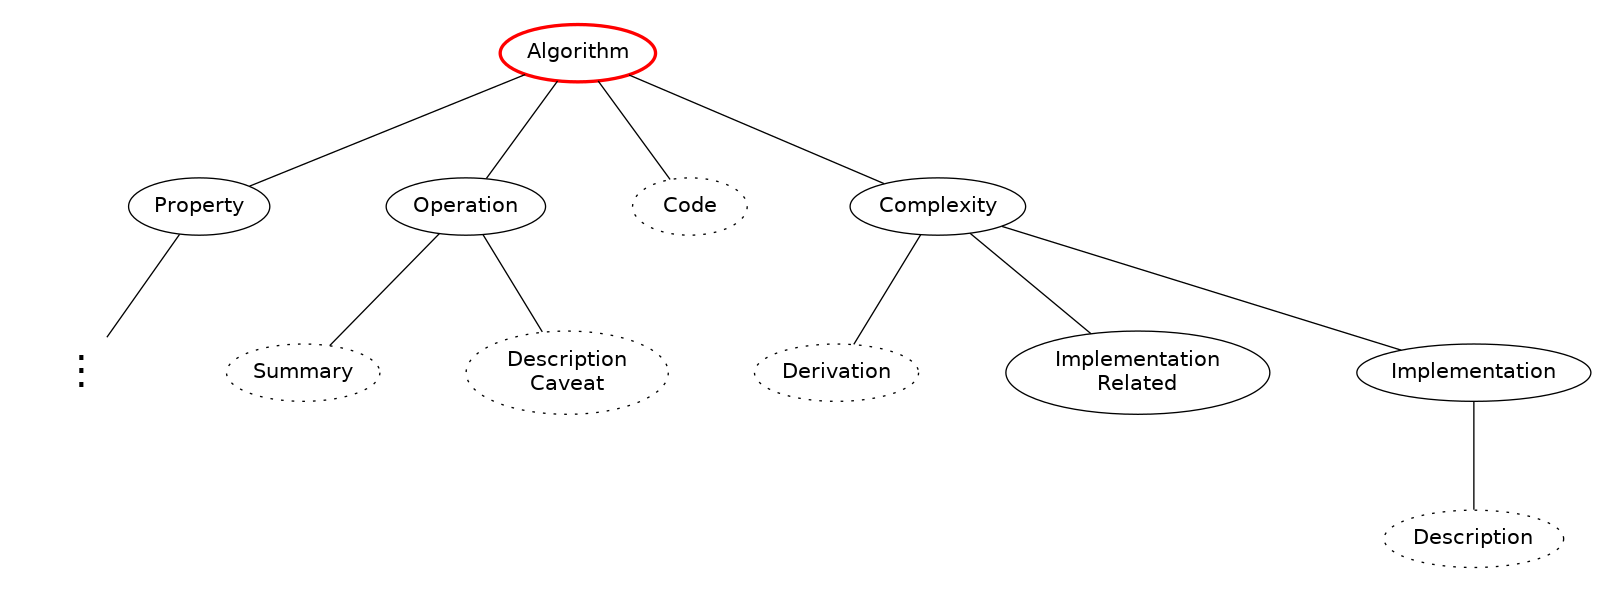
\includegraphics[scale=0.5, trim={0.2cm 0.5cm 0.5cm 0.5cm},clip]{DJK_tree}
\caption{Explanation Tree for Dijkstra's 04}
\label{fig:djk-tree}
\end{figure}

\begin{figure}
\begin{Verbatim}[fontsize=\small,xleftmargin=2ex]
Aspect Algorithm
+- Aspect Operation
|  +- Move Description
|  `- Move InVivo
+- Move Definition @ [Note Sequence,Note Cartoon]
+- Aspect Motivation
|  `- Move Description @ [Note Mathematics]
+- Aspect Disadvantage
|  `- Move Description @ [Note Mathematics]
`- Aspect Operation
\end{Verbatim}
\caption{Rendering of the explanation tree produced by the coding of the
beginning of MS03 given in Table~\ref{tbl:sample}.}
\label{fig:tree}
\end{figure}

The coding system borne out of the data is, in essence, one used to describe a
tree structure. This conclusion was born out of necessity during axial coding
and became the \emph{coding paradigm} for this study. The central problem was to
keep track the different topics each document would discuss throughout their
duration. This led directly to the creation of aspect and structure tags, which
upon retrospection clearly formulate into a tree structure. An
example tree is given below, constructed, by hand, via
graphiz~\cite{Ellson2002}.


Figure~\ref{fig:djk-tree} displays the explanation tree of an explanation
artifact for Dijkstra's algorithm, that has been slightly altered to provide a
useful example. Pentagonal nodes denote aspect nodes, while boxed nodes denote
leaves, and the oval node is the root. We us a vertical ellipses to represent an
arbitrary sub-tree. Italicized text represents a modifier or notation tag that
\emph{has been applied} to another tag. Note that many leaves have been omitted
for space considerations. By observation, a pre-order traversal of this tree
corresponds with a normal reading of the document.

Aspect tags become nodes in the explanation tree, and the aspect is set by the
path to a given node. For example, if the aspect path is \brackets{Algorithm,
  Operation} then the aspect is discussing the ``Operation'' of the
``Algorithm''. Moves are leaves in the tree. If the move occurs in the code
coincident with a structure and aspect tag, then it is represented in the tree
as a leaf of the child aspect, for example the ``Summary'' leaf of the
``Operation'' node. If a move tag appears without an aspect tag, then it
represents a terminal leaf attached to the current node, as shown at the root
node. If a move tag appears coincident with the pop operator then it manifests
as a leaf, on the parent of the current node. This corresponds with popping the
aspect, and then applying the move. Notation tags are represented as terminal
leaf nodes, as seen at ``Code'' in figure~\ref{fig:djk-tree} or attached as
labels to existing nodes or leaves as shown in ``Derivation, Mathematic''.
Modifier tags are represented as labels that are attached to their input tags,
regardless of how those input tags manifest, an example is node ``Implementation
Related''.

Some examples of reading the explanation tree in figure~\ref{fig:djk-tree} are
as follows: Consider the path ``Algorithm, Complexity, Implementation Related'',
this would be read as ``The document is discussing a related implementation of
the algorithm, in terms of its computational complexity''. Another path may be
``Algorithm, Operation, Summary'', this would be read as ``The document is
giving a summary of an operation the algorithm uses''.

\section{Discussion of Results}
\label{sec:dis}
In this section we summarize and interpret the results presented above. In
section \ref{sec:dis:model} we describe the benefits of translating explanation
artifacts into explanation trees. Section \ref{sec:dis:expr} reflects on
supporting varied expressions of like content and section \ref{sec:dis:tail}
discusses the support of tailored, adaptive, explanations. Although we posit
several benefits to using work presented in this paper, all such benefits are
merely conjectures until such a DSL, as is referenced throughout this paper, is
created. \todo{where do we say this line}

The central problem with designing and constructing an explanation-oriented DSL
is translating explanations into an abstract computational model. Several issues
immediately arise with such an approach: 1) What is an \emph{explanation} and
how does one model it as a computational concept? 2) How does one react to user
input? 3) How does one capture varied notation? 4) Similarly, how does one
capture the flexibility and robustness of tailored explanations. Throughout this
section we refer to the \emph{consumer} of an explanation to mean the end
audience for an explanation that the user of the DSL creates.

\subsection{Advantages of an Abstract Model}
\label{sec:dis:model}

% Problem 1
Rather than delving into the yawning maw of philosophy of
explanation~\cite{sep-scientific-explanation} we offload such concerns to the
prospective user's of the DSL. The remaining issues, we believe, are
significantly alleviated with explanation trees.

% Problem 2
In order to support interaction with a consumer a DSL must have an abstract
model with which the user, and consumer may interact with. Explanation trees
directly enable this type of behavior by providing an abstract model of an
explanation artifact.
%
By distilling an explanation artifact into an explanation tree, a user may
create an explanation that matches, and extends, the interactivity with static
documents. For example, a user may want to create an explanation of the
mergesort algorithm; which would correspond directly with a translation of an
explanation artifact to an explanation tree. The user may then anticipate
inquires into other topics related to mergesort but that are not covered in
static documents, such as computational complexity or array data structures.

Because explanation trees are, in essence, abstract models of explanations, one
could imagine the user adding special edges or \emph{links} to support such
inquires. Then if a consumer of the explanation inquired about computational
complexity, the explanation could traverse such a link to the explanation tree
for computational complexity. Such features are simply not possible with
traditional static documents.

Furthermore, the benefits of an abstract model is that one is now able to
compare, abstractly, different explanations for like things. In fact, one may
envision having database of explanations for like things which could be used to
formulate a \emph{general explanation} for a given topic. Such a database would
have more advantages, some of which are described below.

\subsection{Handling Content Expression}
\label{sec:dis:expr}
% Problem 3
A trivial examination of explanation artifacts or any experience in academia
reveals that like things are explained using varied and eclectic notations. The
notations encompassed in the coding system are unlikely to be an exhaustive list
of all such notations.

Content is orthogonal to expression in an explanation tree, thus content may
therefore be separated from notation, and the expression of content in an
explanation tree is extensible. A thorough or meticulous user may wish to create
explanations that can express content with varied notations. Such a user may
provide their explanations with a textual expression, a cartoon expression or a
mathematical formulation, all notations are viable because of the separation of
content and content expression. Such features are currently matched by
traditional static documents. An explanation-oriented DSL, that operates on
explanation trees, could support expressing a single aspect (a single node in
the explanation tree) with different expressions, thereby increasing the options
available to DSL users and explanation consumers.

For example, a DSL user may provide a code based expression for the relax
operation in Dijkstra's algorithm, but they may also provide an auxiliary
cartoon based expression. The addition of an auxiliary expression could then be
requested by an explanation consumer. Technically, the explanation-tree would
simply have another expression tag applied to the same node. This feature, the
ability to express the same content, in many notations, at the request of the
explanation consumer, is only observed in in-person explanations. \todo{this probably
  needs work}

% Problem 4
\subsection{Towards Tailored Computational Explanation}
\label{sec:dis:tail}
The last issue with an explanation-oriented DSL is that of supporting tailored
explanation. This problem essentially boils down to adapting, in real time, to
an explanation consumer. While support for such a feature will hinge on the
interaction semantics available to the consumer, we view explanation trees as
being a significant step in the right direction.

Serving as an abstract model, it becomes possible to collect several explanation
artifacts of like content, much like the data used in this study. By having a
database of such artifacts a user could construct an explanation that draws upon
several explanation artifacts except just one, as is the case with current
static \emph{and} interactive tools. Thus, if a consumer becomes stuck on a
at some point of an explanation, they may switch to the corresponding point in
another explanation and attempt to proceed from there, or consume only that
node, and then return to the previous explanation. While this is still far from
competing with a one-on-one tutorship on the material, such a feature is simply
impossible with static documents and represents a step toward more interactivity.

\section{Conclusion and Future Work}

\todo{write conclusion}
As described in the previous section, we believe that this work offers several
avenues of continued research. First an foremost is to begin writing a DSL based
on the results presented here. Several aspects of the DSL are abstract; for
instance the semantics of interaction, and the user interface. These aspects of
the DSL are likely to remain open questions until an implementation is created. 

The coding system is, admittedly, based on few raw documents. While we reached
saturation with only eleven documents, there is always a risk that the coding
system is not transferable to other computer science content. Thus, more coding,
with varied content is pivotal to validate that the coding system can actually
express radically different content then that which it is grounded in.
\todo{what else?}

\bibliography{XOPbib,eric}
\bibliographystyle{ACM-Reference-Format}

\end{document}
